

\section{Basic notions}
\subsection{Image characterisation}
\begin{qbox}\begin{itemize}
 \item Cite the names of the major image file formats and their main differences. What is DICOM?
 \item Define sampling in numerical images. Define the image resolution. 
\end{itemize}
\end{qbox}
% 
% \subsubsection{Eléments de correction}
% On peut citer les formats jpeg, png, tiff, bmp (bitmap), raw, gif... J'attendais principalement les notions:
% \begin{itemize}
%  \item de compression,
%  \item avec ou sans perte.
% \end{itemize}
% Le format DICOM est un méta-format, principalement utilisé en imagerie médicale, qui permet de stocker des informations sur l'acquisition, les patients, etc...
% 
% Concernant l'échantillonnage,
% \begin{itemize}
%  \item l'échantillonnage spatial définit la pixelisation (donc la résolution si on parle de visualisation ou d'impression, en points par pouces généralement)
%  \item l'échantillonnage en intensité, appelé aussi quantification (des couleurs).
% \end{itemize}

\subsection{Sensors}
\begin{qbox}\begin{itemize}
 \item What is a Bayer filter?
 \item Explain the principles of demosaicing. 
\end{itemize}
\end{qbox}

% \subsubsection{Eléménts de correction}
% Le filtre de Bayer est une matrice de filtres de couleur placée sur un capteur numérique. Il est composé de deux filtres verts pour un rouge et un bleu (passe bandes). Il permet de recomposer une image couleur à partir d'un unique capteur à partir de l'étape appelée demosaicage (demosaicing en anglais), qui consiste (de manière basique) à réaliser une interpolation des pixels non connus.

\subsection{Image processing}
\begin{qbox}
\begin{itemize}
 \item Define the operation of histogram equalization. 
 \item What is the difference with histogram stretching? 
 \end{itemize}
 \end{qbox}
 
 \begin{qbox}
 \begin{itemize}
 \item From the mathematical definition of the derivative, explain the construction of the gradient operator, and then of the Laplacian. 
 \item Cite some method for contours detection, and list their pros and cons. 
\end{itemize}
\end{qbox}

% \subsubsection{Eléménts de correction}
% L'égalisation d'histogramme est une opération permet d'ajuster le contraste d'une image numérique en construisant une transformation à partir d'un histogramme cumulé (équivalent à une fonction de répartition). L'objectif est d'obtenir une densité de probabilité en loi uniforme. 
% 
% L'étirement d'histogramme a un but identique, mais la transformation d'intensité est linéaire. Cette méthode est sensible et peu efficace lors de la présence de valeurs extrêmes.

\section{Open question}

\begin{qbox}
 The Fig. \ref{fig:exams:2016:theorique:retine}  shows a human retina (eye fundus). Propose a method for segmenting:
 \begin{itemize}
  \item the vessels,
  \item the optical nerve (bright disk).
 \end{itemize}

 Justify your choices. Indicate all elements that seem important and the way to deal with them. Look carefully at the shapes and intensities of objects you need to segment.

 For your record, ophthalmologists need to measure the diameter and the circularity of the optical nerve, as well as the length and the number of vessels (branches, tortuosity...).
 
\end{qbox}

\begin{figure}[H]
	\centering\caption{Human retina.}%
	\subfloat[Color image.]{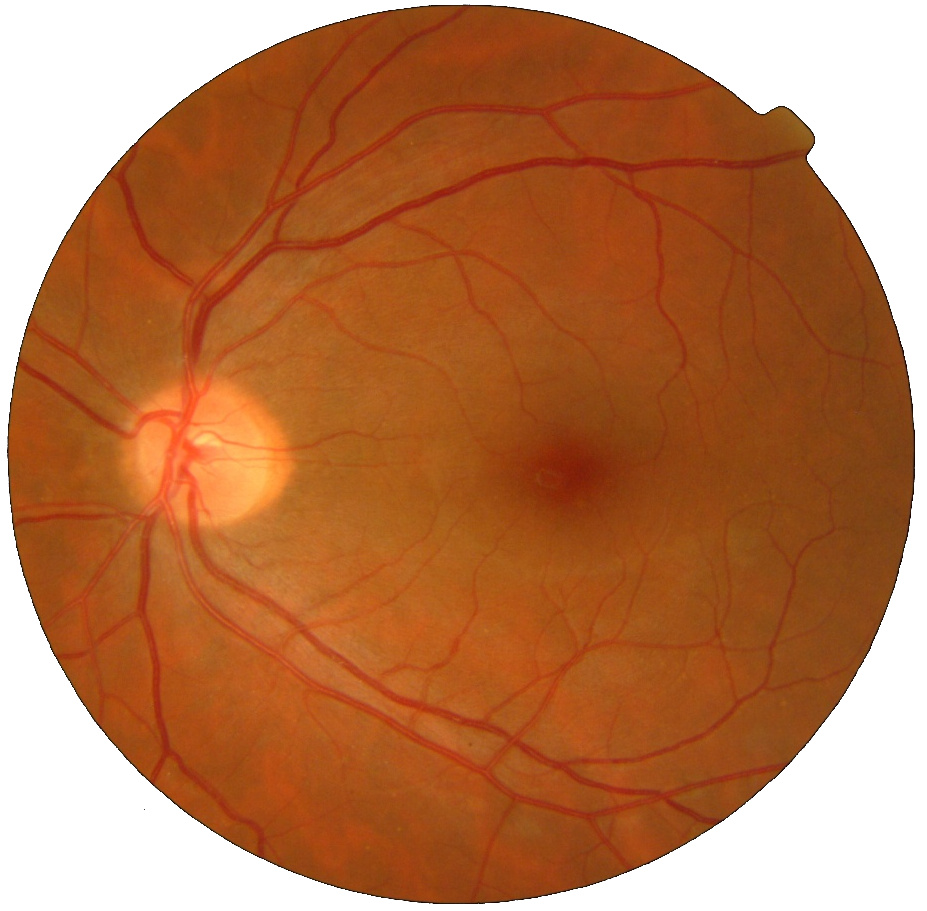
\includegraphics[width=.45\linewidth]{retine.jpg}}\hfill
	\subfloat[Red channel.]{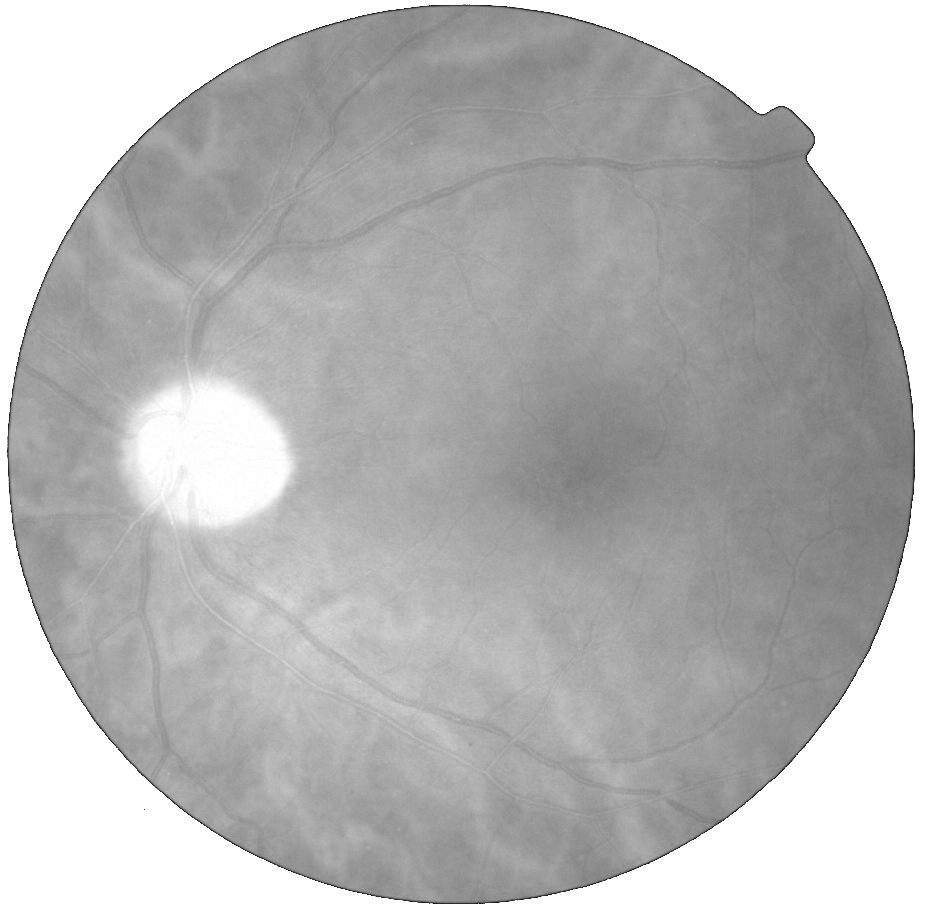
\includegraphics[width=.45\linewidth]{retine-R}}
	
	\subfloat[Green channel.]{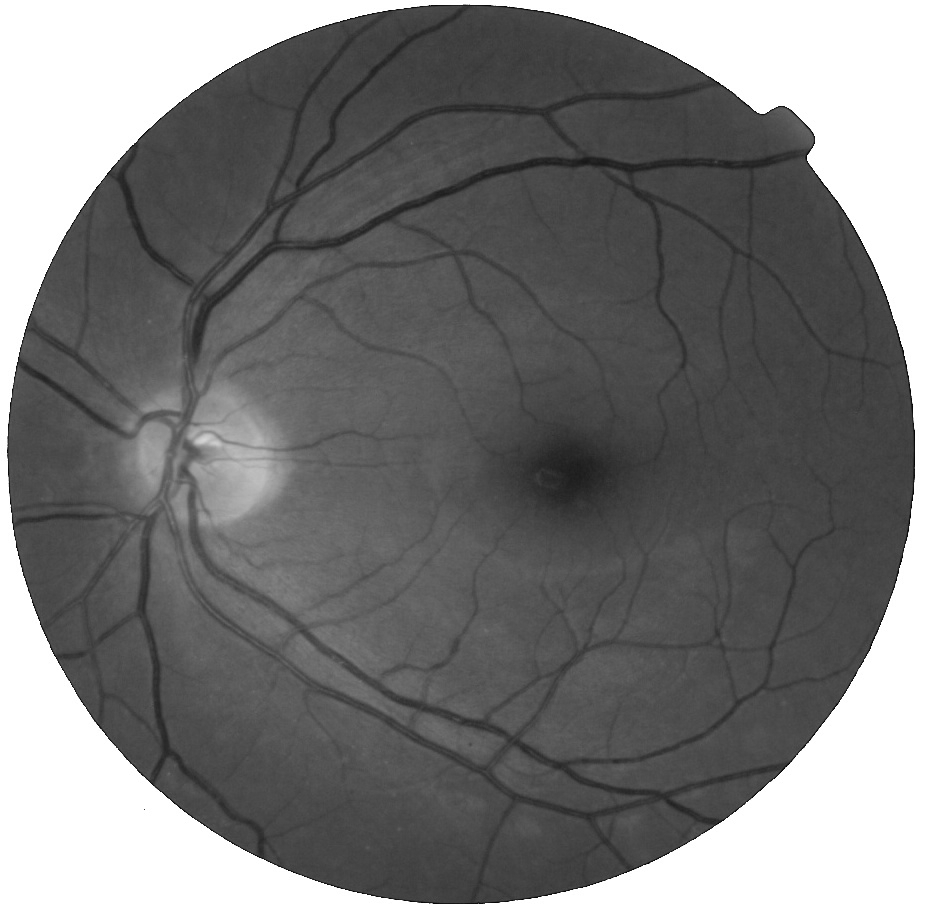
\includegraphics[width=.45\linewidth]{retine-G}}\hfill
	\subfloat[Blue channel.]{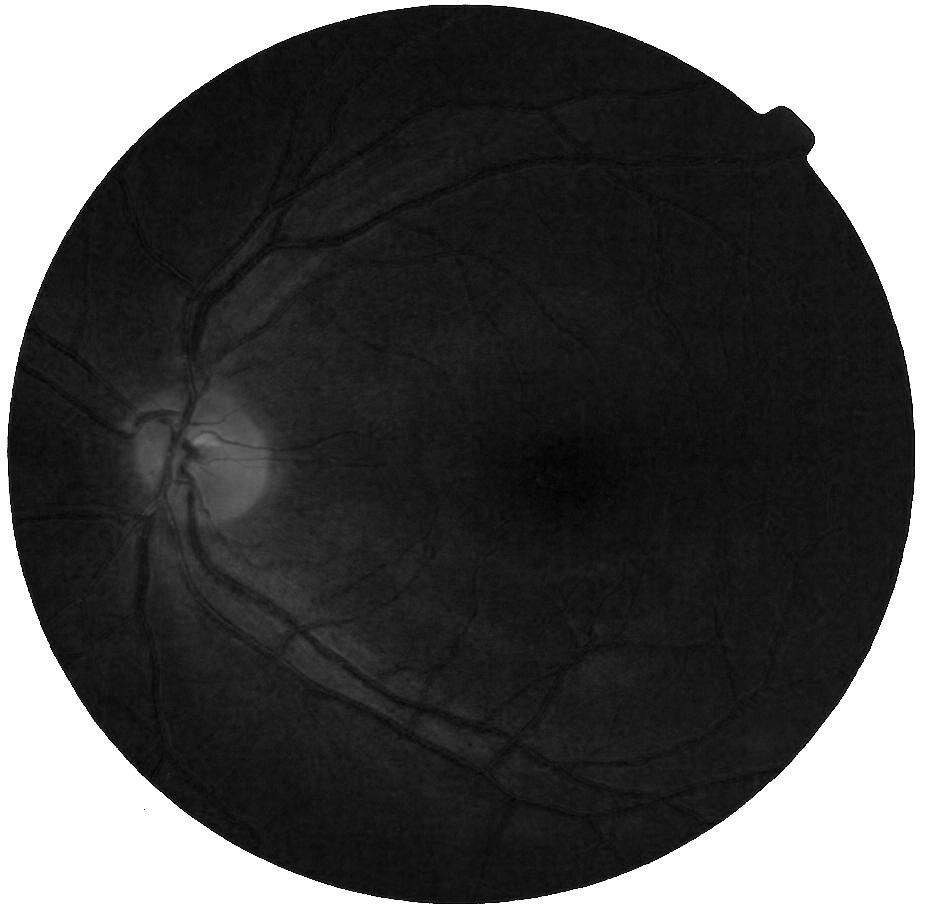
\includegraphics[width=.45\linewidth]{retine-B}}
	\label{fig:exams:2016:theorique:retine}
\end{figure}

% \vspace{1cm}
% \subsubsection{Eléments de correction}
% Il fallait évidemment noter que le canal vert était adapté pour la segmentation des vaisseaux, le canal rouge pour la segmentation du nerf optique. Le premier réflexe est donc d'appliquer un seuillage. Sur les 7 points, vous aviez 4 si ces éléments étaient présents.
% 
% Ensuite, j'ai ajouté des points sur les éléments pertinents mis en avant:
% \begin{itemize}
%  \item présence de la tache sombre au centre (macula), et donc tentative de suppression,
%  \item forme des vaisseaux (sombres, filiformes, connectés), et méthodes pour essayer de les séparer du reste (parties connectées les plus grandes, touchant les bords)
%  \item présence de bruit
%  \item région d'intérêt (élimination du blanc autour de l'image)
%  \item charactérisation du disque du nerf optique (critères de circularité, diamètre de feret, etc.)
% \end{itemize}
% 
% Vous n'aviez évidemment pas toutes les connaissances pour arriver à segmenter cette image parfaitement, j'ai donc plus noté sur les objectifs que vous présentiez, plutôt que sur la manière de le faire. 
% 
% Les méthodes actuelles se basent sur des filtres gaussiens orientés dans une direction, que l'on applique sur toutes les directions pour cumuler les résultats et extraire les parties linéaires. Il est possible également de faire de la croissance de région à partir de points facilement détectables, en profitant de la connectivité des vaisseaux (tracking).
